\documentclass[twocolumn, 10pt]{article}
\usepackage{listings}
\usepackage{xcolor}
\usepackage{graphicx}
\usepackage[sorting=none]{biblatex} %Imports biblatex package
\graphicspath{ {./images/} }
\addbibresource{sample.bib} %Import the bibliography file



\begin{document}
\lstset{language=C,keywordstyle={\bfseries \color{blue}}}

\title{%
 \textbf{Auto: an open protocol for the autonomous metaverse }
}
\author{Jeremiah Wagstaff \\
\textit{jeremiah@autonomys.net}
}

\date{}

\maketitle

\begin{abstract}
\textit{The metaverse does not yet exist. Instead we have a series of fragmented virtual worlds that cannot communicate with each other. This is because we lack an open standard for interoperability. To resolve this challenge we propose auto, an open protocol for the autonomous metaverse. Auto allows developers to easily build interoperable virtual worlds using existing web technologies. These worlds are autonomous, meaning they are user-centric, self-sovereign, and permissionless -- in the spirit of the original web. Auto allows for the emergence of the autoverse, an interoperable network of autonomous virtual worlds, owned and controlled by users, not corporations.}
\end{abstract}

\section{Problem}
The metaverse, in the form of single interoperable network of immersive virtual worlds, does not yet exist. Instead, we are seeing an increasing number of \textit{closed metaverses}. This is because existing worlds are fragmented across platforms, each a walled garden, often controlled by a single company like Meta, Roblox, or Epic. Users cannot freely traverse these worlds, as their identities and virtual assets are not portable across platforms. Developers cannot yet easily build these worlds on their own, forcing them to rely on platforms for distribution and monetization.

The key problem is that there does not yet exist an open standard for creating interoperable virtual worlds. Instead, today’s virtual worlds are built using proprietary game engines like Unity and Unreal, in accordance with the rules of each individual platform. This sad state of affairs stands in stark contrast to the web, which is based on royalty-free, open standards like HTTP and HTML, alongside the open distribution model of the browser.

If we fail to deliver open standards for the metaverse, fragmentation will eventually lead to consolidation and monopolization around a single dominant platform. This platform will effectively become the metaverse. As virtual worlds consume an increasing fraction of our time spent online, control over the metaverse will be tantamount to control over the Internet, and our increasingly digital lives.

\subsection{The Open Metaverse}
To address this problem, a growing number of engineers, entrepreneurs, and evangelists across a diverse array of industries and backgrounds have organized into a network of standards bodies, working groups, and foundations. They all share the common goal of defining a set of open standards for the open metaverse. Open standards would enable interoperability and prevent platform lock-in for both developers and users. To date, most of these standards have originated from two institutions.

The Khronos Group has developed several royalty-free open standards for 3D graphics and Extended Reality (XR) devices, including the Graphics Language Transmission Format (glTF), the WebGL and WebGPU 3D graphics APIs, and the OpenXR device API \cite{khronos}. The World Wide Web Consortium (W3C) has created the WebXR device API, the WebAssembly (WASM) portable execution format, and the Decentralized Identifier (DID) specification \cite{W3C}. While these efforts have succeeded in defining many of the key primitives required for an open metaverse, we are still missing an overarching protocol which weaves them together into a single coherent system.

\subsection{Autonomous Worlds}
Web3 provides inspiration for how such a protocol might work in practice. Smart contract blockchains like Ethereum have defined interoperability frameworks around standards like ERC-20 and ERC-721, which work across a permissionless global computer running untrusted user-generated code \cite{Buterin2013}. In this light, Ethereum may be understood of as an abstract public metaverse. Projects such as Dark Forest, Cryptovoxels, and Decentraland have taken this idea to the next level, by defining 2D and 3D virtual worlds that live inside of the Ethereum blockchain.

The idea of blockchain-based virtual worlds defined by smart contracts has recently been formalized as \textit{autonomous worlds} \cite{AutonomousWorlds}, which express the key feature of \textit{permissionless interoperability}. Autonomous worlds are user-centric, self-governing, and inherently moddable. Just like the real world, no one has to ask permission to play by their own house rules, while everyone has the freedom to adopt whichever rules they like best. Frameworks like MUD have further encapsulated the idea of autonomous worlds by adapting the Entity-Component-System (ECS) design pattern widely used in the video game industry to Solidity-based smart contract development, transforming the Ethereum \textit{world-computer} into an autonomous \textit{world-engine} \cite{MUD}.

Perhaps surprisingly, decentralized communication protocols have also been used to create autonomous worlds \textit{without a blockchain}. Thirdroom is a network of immersive virtual worlds built using the Matrix protocol \cite{ThirdRoom}. It also employs the ECS pattern, but instead runs the world-engine within the browser through WebAssembly. This allows web developers to define worlds in Javascript, while still supporting untrusted, user-generated code. Thirdroom demonstrates that blockchains are not strictly required for autonomous worlds.

What is needed is a single unified architecture for autonomous worlds that works across protocols. Like the web, it must be flexible, allowing for a diverse ecosystem of programming languages, development frameworks, and user-facing platforms to emerge. Like web3, it must embrace and enshrine the notion of peremissionless interoperability. 

\section{Solution: Auto Protocol}
To address these challenges, we propose \textit{auto: an open protocol for the autonomous metaverse}. Auto allows for the emergence of \textit{the autoverse}, a massively-scalable distributed network of autonomous virtual worlds. All worlds across the autoverse are permissionlessly interoperable, allowing them to be freely defined by developers, while ultimately controlled by their users, \textit{not corporations}. 

\subsection{Guiding Principles}

Auto is based on the following core principles.

\begin{enumerate}
    \item \textbf{User-Centric:} identity should be self-sovereign and portable across worlds, allowing each user to be a first-class citizen of the system, rather than a servant to their platforms.
    \item \textbf{Web3 is Opt-In:} developers should have the freedom to build worlds as they see fit, without sacrificing interoperability, making blockchains and peer-to-peer networks optional.
    \item \textbf{Back-End Agnostic:} the protocol should be modular, supporting existing storage, compute, and networking back-ends; whether they be centralized, distributed, or decentralized.
    \item \textbf{Decoupled View Layer:} the underlying world-engine should be cleanly separated from any game engine or rendering pipeline, following the Model-View-Controller (MVC) pattern.
    \item \textbf{Web-Based:} the protocol should be built from existing web-standards, allowing it be backwards-compatible with the web and natively cross-platform through the browser.
\end{enumerate}
\\\\
Auto provides an open platform for innovation, which will drastically lower the barriers to entry for world-building and unlock a new wave of innovation across the emerging field of immersive design.  A common framework for interoperability will also allow the autoverse to benefit from the kinds of network effects that helped to propel the early growth of the web.

\begin{figure}[h]
    \centering
    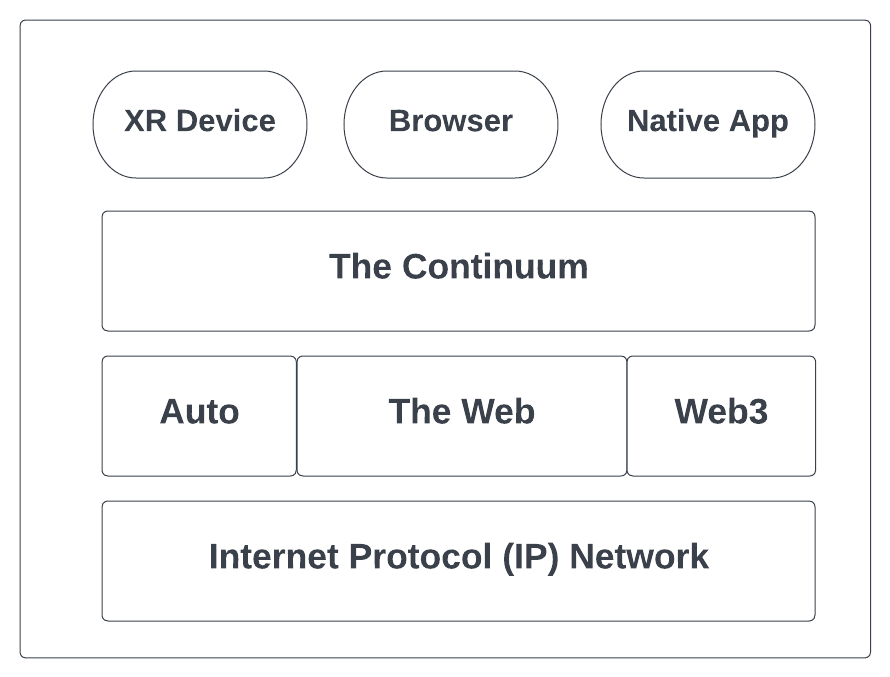
\includegraphics{images/autoverse.png}
    \caption{The Autoverse}
    \label{fig:my_label}
\end{figure}

\subsection{Non-Goals}

At the same time, its worth stating what auto is not.

\begin{itemize}
    \item \textit{Auto is not the web}. While it may be exposed over the web and experienced within a browser, it does not seek to become a new W3C standard.
    \item \textit{Auto is not a web3 protocol}, though it does allow worlds to leverage existing Web3 protocols for decentralized storage, networking, and compute.
    \item \textit{Auto is not a blockchain}, though worlds may employ blockchains to agree on critical global state, such as ownership over identity or virtual assets.
    \item \textit{Auto is not a consensus protocol}, as the autoverse has no canonical global state. Instead, each world chooses its own \textit{off-the-shelf} consensus.
    \item \textit{Auto is not a singleton network}. Instead, each world has its own network, with optional sub-nets, which are not necessarily connected.
    \item \textit{Auto is not a programming language}, though it may be implemented in many languages, while inspiring new languages for expressing worlds.
    \item \textit{Auto is not a framework}, though it may leverage existing web frameworks and game engines, while inspiring new \textit{world-building} frameworks.
\end{itemize}

\subsection{The Autonomous Stack}
Auto is an application layer protocol, designated by the \lstinline{auto} URI scheme, which runs across the Internet Protocol (IP) network. It includes a set of sub-protocols for describing, running, and interacting with autonomous virtual worlds. The auto protocol is organized according to the autonomous stack. It consists of seven layers, starting from the top:
\begin{enumerate}
    \item \textbf{Device}: Supports desktop, mobile, console and all OpenXR compatible hardware devices.
    \item \textbf{Interface}: Renders in any WebXR compatible browser or OpenXR compatible game-engine.
    \item \textbf{Application}: Orders world-messages and runs experiences within the VECS world-engine.
    \item \textbf{Network}: Syncs world-state, world-assets, and propagates world-messages over the IP suite.
    \item \textbf{Naming}: ANS maps human-readable names to content-addressed decentralized identifiers.
    \item \textbf{Identity}: assigns decentralized identfiers to all autonomous agents, worlds, and world-entities.
    \item \textbf{World}: defines a world-interface for all world-entities according to the VECS world-model.
\end{enumerate}
Auto is defined through a set of core frameworks for interfacing with the various layers of the autoverse.  
\\\\
\textbf{Hyperspace} is a conceptual framework based on the Virtual ECS (VECS) world-model. It provides a unifying theme for the auto core protocol.
\\\\
\textbf{The Continuum} is an interconnected web of worlds and experiences that run across the autoverse. It serves as the shared user interface for auto.
\\\\
\textbf{Lattice} is a modular framework for world-builders. It allows developers, designers, and modders to craft and remix immersive virtual worlds and experiences.
\\\\
\textbf{Autonomys} is a distributed organization that maintains the auto protocol and manages the auto standards process via the nomic governance protocol.

\section{Building Blocks}
Before diving into auto, it is worth reviewing the patterns and primitives from which it is composed. 

\subsection{Entity-Component-System}
ECS is a design pattern employed in video game development for efficiently managing objects in virtual worlds \cite{Entitiies}. Unlike object-oriented programming paradigms, which treat every \textit{thing} as an object, ECS treats every thing as an \textit{entity}. ECS favors composition over inheritance, allowing entities to be assembled, like virtual Lego's, from \textit{components} of structured data and \textit{systems}, expressed as pure functions. Together, components and systems define behaviors for different types of entities. ECS allows developers to build complex worlds from a handful of behaviors, while remaining extensible post-launch. When combined with a secure execution environment, anyone may extend or \textit{mod} these worlds. Different worlds which share the same ECS engine are interoperable, allowing entities to freely move between them. Many existing game engines already support ECS. 

\subsection{Decentralized Identifiers}
Decentralized Identifiers (DIDs)  are a new type of identifier, that enables verifiable, decentralized digital identity \cite{reed2020decentralized}. DIDs allow users of online systems to create and manager their identities entirely on their own. While they rely on public key cryptography for security, they do not depend on blockchains or peer-to-peer networks at all. DIDs are extremely flexible, allowing for interoperability across centralized systems, federated networks, and Web3 protocols. The specification supports using DIDs for identity, naming, addressing, authentication and authorization in a trustless, secure, and privacy-preserving manner. DIDs allow ECS entities to autonomously manage their own unique identifiers and addresses. 

\subsection{Capabilities Based Security}
A capability is an unforgable token of authority which an entity may use to access certain rights within a computing system. Capabilities are used to secure systems comprised of mutually untrusting entities. They follow \textit{the principle of least privilege}, which states that an entity should only have access to the system information and resources required for a specific purpose \cite{saltzer1975protection}. They are often contrasted with access control list (ACLs), such as the UNIX permission system. Capabilities may be granted, modified, delegated, and revoked across entities within the system, according to their own capabilities. Since DIDs also support capabilities, they allow each ECS entity to autonomously manage its own security.

\subsection{Actor Model}
The actor model is a theoretical framework of concurrent computation that treats actors as the basic building block of distributed systems \cite{hewitt1973universal}. Actors are abstract processes, or entities, that communicate through message passing. In response to a message, an actor may act on its private state, spawn new actors, or send new messages. Actors remove the need for lock-based synchronization, allowing them to be used for massively-scalable, asynchronous distributed systems like E-mail and cellular networks.

\subsection{Existing Web Standards}
Web standards allows the browser to serve as the default cross-platform interface for users and a permissionless distribution platform for developers.
\begin{itemize}
    \item \textbf{WebCrypto} provides DID security primitives
    \item \textbf{WebRTC} provides a realtime network interface
    \item \textbf{WASM} provides a secure, performant runtime
    \item \textbf{WebGL/WebGPU} provide the graphics APIs
    \item\textbf{glTF/GLB} provide a standard 3D file format
    \item \textbf{WebSG} provides a 3D SceneGraph API
    \item \textbf{WebXR/OpenXR} provide XR device APIs
\end{itemize}

\section{Hyperspace}

Auto is built around the unifying theme of \textit{hyperspace} and is organized according to a modular \textit{hyperstack}.  
\begin{enumerate}
    \item \textbf{HyperID}: a method for identifying, addressing, and describing entities across virtual worlds
    \item \textbf{Hypertime}: a web assembly runtime environment that implements the VECS world-engine
    \item \textbf{Hyperclient}: a modular software application that allows worlds to run locally on a host device
    \item \textbf{Hyperspace Relay Protocol}: HSRP is a consensus-agnostic real-time network protocol
    \item     \textbf{Hyperspace Markup Language}: HSML maps VECS entities to HTML web components
\end{enumerate} 
Although auto is not the web, it may be understood in similar terms. If hypertext is a way to instantly traverse a collection of virtual documents across the web, then \textit{hyperspace} is a way to instantly traverse a collection of virtual \textit{spaces} across the autoverse. It transforms web links into hyper \textit{portals}, web pages into hyper\textit{ spaces}, and web sites into hyper \textit{worlds}.

\subsection{Hyperspace Identifiers}

 Unlike the web, auto ensures users are first-class citizens of the system through self-sovereign \textit{Hyperspace Identifiers}. The hyperspace \textit{world-model} follows the ECS adage \textit{everything is an entity}. However, unlike most ECS frameworks, which treat entity ids as integers, similar to a database primary key; auto follows the DID spec, and instead manages entities as decentralized identifiers across a distributed global name-space. This means that every \textit{thing} in the autoverse is both an entity and a DID, including all worlds, objects, and autonomous agents.

Each world is identified by its DID URL, derived as the content-addressed hash, or \textit{content identifier} (CID), of its DID \textit{controller}, typically a public key. Spaces within worlds are identified by DID \textit{path}, as the CID of the \textit{path name}. Exact locations within a space are designated by DID \textit{fragment}, in accordance with the spatial coordinate system of each individual world. Each in-world entity is a delegate DID in the form of a new DID \textit{subject}, managed by the world’s DID controller. Entities are identified as the CID of the the entity index concatenated with the world’s DID, allowing entity URLs to be treated as fragments within the world's URL. 

\begin{figure}
    \centering
    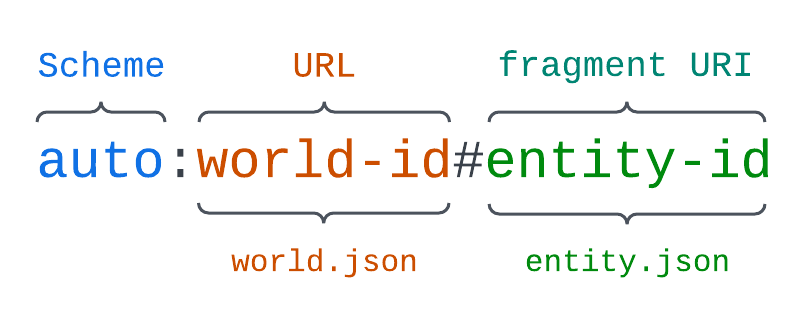
\includegraphics[width=\columnwidth]{images/hyperid.png}
    \caption{HyperID Syntax}
    \label{fig:my_label}
\end{figure}

Each world is defined by its DID \textit{document}, which encapsulates a \textit{world-interface} describing the systems, components, and other metadata attached to it. The world-interface is represented as \textit{world.json} file, which is tracked with a version-controlled Git repository, allowing each world to be treated as series of immutable CID snapshots. If each snapshot is signed by the DID public key, anyone can verify that they are on a valid version. 

Each autonomous agent with the autoverse also has its own independent DID, which is portable across worlds. These includes users, organizations, smart contracts, bots, and embodied AIs. Agents are also identified by a DID URL derived from the controller CID. Each agent also has a DID document which describes their public profile, such as their handle, avatar, and other metadata. When agents enter worlds a proxy \textit{world-entity} is spawned on their behalf. Agents may also be used as proxy controllers for other top-level DIDs, such as worlds or other agents. 

To make DIDs user-friendly, any DID URL may be mapped to a human-readable name using a verifiable data registry, such as the Domain Name System or a public smart contract blockchain, through the Autonomous Name System (ANS). The DID URL resolves to the underlying DID document. Authenticity is verified by signature using the DID public key, while pointing to the last verifiable snapshot.

\subsection{Hypertime}

Worlds run in \textit{hypertime}, the \textit{hyperspace web assembly runtime}, which replaces the V8 javascript engine with the \textit{Virtual ECS} (VECS) \textit{world-engine}, allowing anyone to define and extend worlds with user-generated scripts in any WASM friendly language. VECS is an abstract model of computation that encapsulates the ECS pattern under an actor model of concurrency within a virtual machine. It allows an unbounded set of replicated state machines, each reflecting a unique virtual world, to safely communicate over an asynchronous network. 

Worlds are just collections of entities, meaning that every abstract thing within a world is tracked as an entity. Each entity is referenced by a HyperID, which maps to a set of components and systems registered to the world, reflecting the entity's capabilities. Each entity is also an actor, which may be addressed by its HyperID and called through any related system. When called with a message, the entity may modify its own state, spawn new entities, or send messages to other entities. 

\begin{figure}
    \centering
    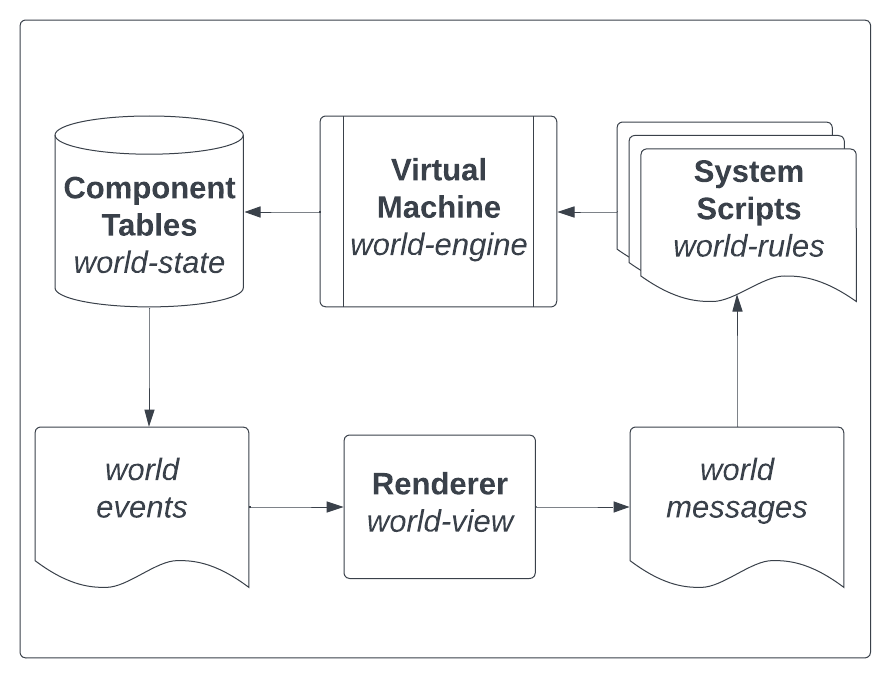
\includegraphics{images/vecs.png}
    \caption{VECS World-Model}
    \label{fig:my_label}
\end{figure}

For each world, VECS manages the world-state of all child entities in response to abstract messages, by executing system calls, updating component state, and emitting events, all in accordance with the world-interface. For performance proposes, all world-state is managed in-memory, although a hyperclient may provide a persistent storage back-end, such as relational database. VECS combines a pure ECS back-end with the MVC pattern, by decoupling the notion of a rendering or view layer into a separate scene-graph that is updated through events. 

VECs is described as a world-engine rather than a game-engine to highlight it’s more fundamental purpose of managing open worlds, which often lack the clear goals found in video games. However, VECS could still be viewed as a bare-bones game-engine, similar to projects like BitECS, Flecs, or Bevy, which also follow the ECS pattern. The key distinction is that they are all restricted to one specific language, while assuming the code used for ECS systems is trusted. VECS instead works with untrusted code, written in any language that compiles to WASM, making it more similar to virtual machines used by smart contract blockchains. Regardless of naming, VECS may still be used to implement in-world games without precluding its use alongside popular tools like Unity, Unreal, or Godot.


\subsection{Hyperclient}

A hyperclient is a modular piece of software that embeds a Hypertime Virtual Machine (HVM) within a larger runtime environment. It mediates access to network interfaces, the file-system, and other system resources by providing a set of runtime APIs that allow developers to interact with the HVM, client modules, and back-end services. Auto is agnostic to the underlying consensus, storage and networking protocols, so long as they adhere to its interfaces. It embraces the provider pattern by supporting different implementations for each module. 

\begin{figure}[h]
    \centering
    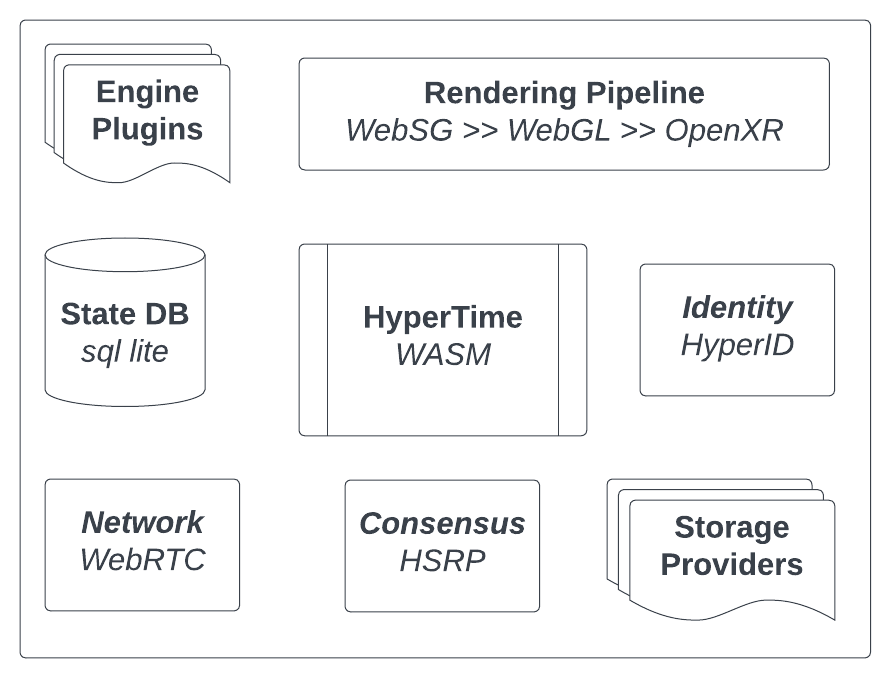
\includegraphics{images/hyperclient.png}
    \caption{Hyperclient Architecture}
    \label{fig:my_label}
\end{figure}

\begin{itemize}
    \item \textbf{Identity}: exposes a secure cryptographic key store for DIDs. HyperID is the default provider.
    \item \textbf{Network}: exposes host networking interfaces. HTTP and WebRTC are the default providers.
    \item \textbf{Storage}: exposes a distributed storage API with a local backup. Gaia is the default provider.
    \item \textbf{Consensus}: mediates network messages to the HVM. Automerge CRDT is the default provider.
    \item \textbf{Runtime}: exposes the system and event APIs of the HVM. Hypertime is the default provider.
    \item \textbf{Database}: exposes a local database to the HVM. SQL Lite WASM is the default provider.
    \item \textbf{Scene-Graph}: exposes an in-memory 3D scene-graph. Default provider is WebSG.
    \item \textbf{Graphics}: exposes low-level host graphics APIs. Default provider is WebGL.
    \item \textbf{Rendering}: exposes an XR-compatible 3D rendering engine. Default provider is three.js.
    \item \textbf{Device}: exposes XR and browser devices APIs. Default provider is WebXR.
\end{itemize}

\subsection{Hyperspace Relay Protocol}

 While Hypertext Transfer Protocol (HTTP) enforces a client-server architecture through the browser, \textit{Hyperspace Relay Protocol} (HSRP) allows hyperclients to communicate directly with one another. HSRP allows clients to maintain the real-time state of worlds and spaces. It runs over the WebRTC network transport, providing audio and data channels directly between clients in the same spaces. HSRP supports multiple network topologies, including peer-to-peer, client-server, and several others. 
 
 Each world typically has one global WebRTC gossip network for syncing the canonical world-sate and broadcasting world messages, along with any number of smaller mesh networks for sharing real-time audio and location data amongst peers within the same space. HSRP is agnostic to the underlying consensus protocol used for ordering messages, leaving this decision up to each world-builder based on their security model. Options include central servers, Lamport clocks, Conflict-Free Replicated Data Types (CRDTs), and leader election protocols like Tendermint and Nakamato consensus.

 \begin{figure}
    \centering
    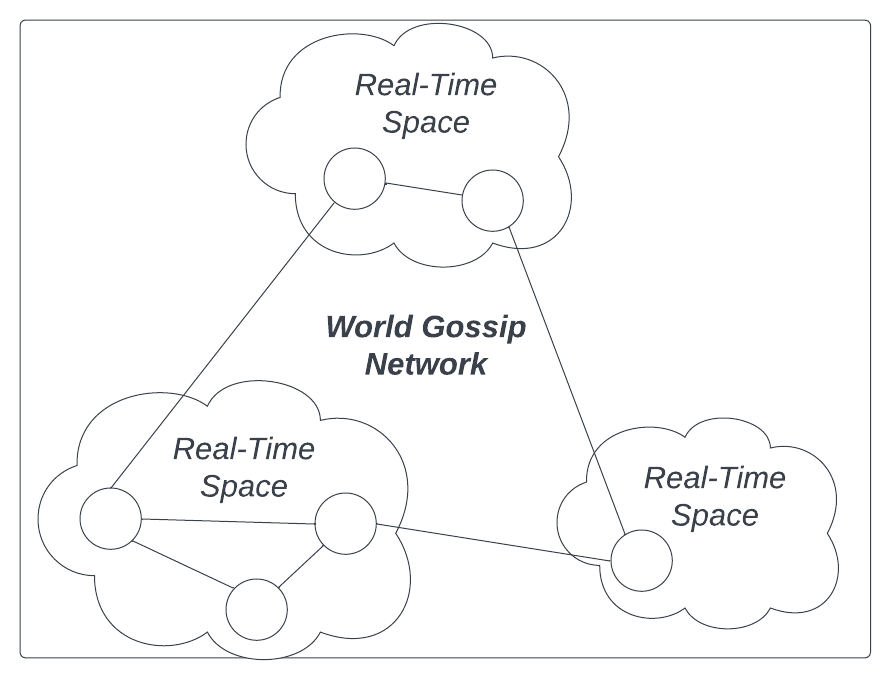
\includegraphics{images/hsrp.png}
    \caption{HSRP across Hyperclients}
    \label{fig:my_label}
\end{figure}

\subsection{Hyperspace Markup Language}

While web pages are expressed in Hypertext Markup Language (HTML) for the document object model (DOM), hyper spaces are defined using \textit{Hyperspace Markup Language} (HSML) for a WebSG \textit{hypergraph}. HSML is a superset of HTML that encapsulates VECS entities as web components. Component libraries are generated dynamically from a world-model. They are expressed declaratively, like standard HTML, modified via CSS properties, and made interactive with javascript. HSML is inspired by earlier immersive web frameworks like JanusVR, A-frame, and Lume. It differs by cleanly separating the ECS from the notion of a browser and the DOM. 

\section{The Continuum}

The continuum is the interoperable \textit{web of worlds} built on auto, where each world represents a distinct dimension of the autoverse. Worlds may vary in their back-end representation, employing different 2D or 3D coordinate systems, while ranging in scale from individual spaces to cities, planets, or entire virtual universes. Each user may experience the representation of a world in a different manner, based on their chosen client and rendering configuration. 

\subsection{World Experiences}

Worlds serve as distributed software containers, whose core logic may be extended with any number of immersive experiences. These might include massively-multiplayer games and open sandboxes, real-time social gatherings and live public events, virtual meeting rooms and co-working spaces, and immersive stores for virtual and physical content. Many of these experiences already exist today as closed monolithic apps, rather than open modular worlds. Auto provides an alternative model that legacy platforms and apps may migrate towards, or risk being overtaken by the next wave of builders.

\subsection{User Generated Content}

Worlds may also support extensions through user-generated-content, in the form of 3D models and scenes. Since auto supports glTF, it works with the entire suite of existing design software, game engines, asset stores, and emerging AI co-creation tools; allowing anyone to easily create and add their own content. 

\subsection{User Generated Scripts}

The continuum takes modding to the next level, since auto allows developers outside the core team to extend both the content and logic of a world \textit{without having to ask permission}. This makes world-building \textit{composable}, as new features and experiences may be layered on top of one another, while allowing users to participate on an opt-in basis. Since auto is interoperable, these experiences may be re-used across worlds which share the same base rules. To promote this pattern, auto includes a standard library of worlds, components, and systems. 

\begin{figure}
    \centering
    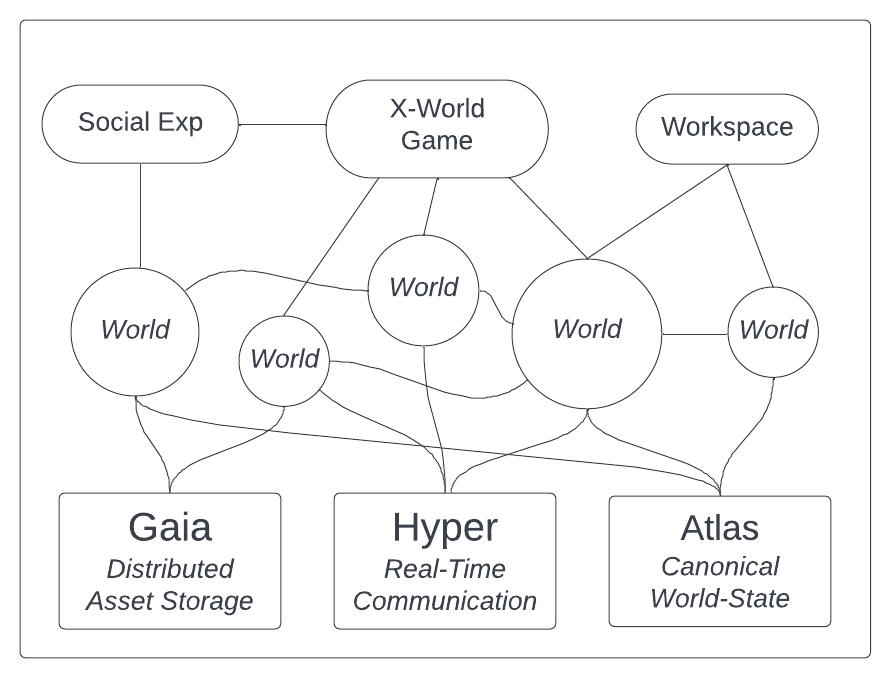
\includegraphics{images/continuum.png}
    \caption{The Continuum}
    \label{fig:my_label}
\end{figure}

\subsection{Trustless Interoperability}

Web3 platforms may be used to enhance composability and interoperability across worlds by making it \textit{trustless}. This allows users to freely traverse worlds by utilizing their identities as digital passports, while taking their virtual belongings with them. Web3 also unlocks new types of worlds that could not exist before. Perlin worlds, could procedurally generate infinitely large, random virtual frontiers, with hidden treasures scattered throughout \cite{perlin1985image}. When extended with zero-knowledge proofs, users could explore these worlds in an efficiently verifiable manner, allowing them to \textit{mine the metaverse} through ordinary play.

\subsection{Pioneer}

Pioneer is a cross-platform application that serves as the preferred world-browser for the continuum. It is inspired by the Steam launcher, and allows users to more easily discover, install, and run worlds natively, vastly improving the user experience. Similar to Ethereum’s Myst browser, it also allow users to easily run light clients of popular Web3 protocols for connected worlds.

\section{Lattice}
Lattice is an open-source framework for world-builders. It allows developers, designers, and modders to craft and remix immersive virtual worlds and experiences. World-building is more art than science, and should follow the creative process. Each world should begin as a concept and story, before moving into visual design, modeling, and finally scripting.

\subsection{Hyper}
Hyper is a cross-platform runtime environment that implements the full hyperstack, providing the reference implementation of auto. It presents a bare-minimum, unopinionated developer framework, inspired by Node.js, which may be used directly to create and run worlds, or as a core component for more sophisticated frameworks. Hyper is written in Typescript for the browser, though it can also be packaged for mobile, desktop, or server envrionments.

\subsection{Gaia}
Gaia is a distributed world manager, inspired by NPM, that provides an asset storage layer for auto. It consists of a command line interface and an online public database of worlds. Gaia allows developers to quickly scaffold worlds, before packaging them for hyperclients. World assets consist of a variety of content types that adhere to the glTF standard such as 3D models, textures, audio files, and scripts. Gaia supports multiple providers, including cloud storage like AWS S3; distributed file systems like IPFS, and archival storage networks like Arweave and Subspace.

\subsection{Atlas}
Atlas is a standard interface for defining VECS-compatible smart contracts for world systems and components. It is inspired by the MUD framework on Ethereum, but extends it to be chain-agnostic, allowing for interoperable entities across networks. Atlas gives developers the flexibility to decide which entities should to be tracked on-chain and which may be tracked off-chain. This allows smart contract blockchains, like Ethereum and Solana, to be used as a root of trust for critical entities within auto, such as identities, in-world objects, and financial assets.

\subsection{Mythic} 
Mythic is an isomorphic world-scripting language. It is a statically-typed, resource oriented programming language, purpose-built for defining autonomous worlds. It combines elements of Solidity and Javascript, making it familiar to both smart contract and web developers. It also includes VECS compliant semantics and keywords for defining the components, systems, archetypes, and entities that make up a world. Mythic compiles to WASM, making it isomorphic, allowing it to run off-chain, within a hyperclient, or on-chain within a smart contract blockchain with a WASM VM, such as Subspace or Near. 

\subsection{Asimov}
Asimov is full-stack, batteries-included framework for composing worlds within the continuum. It is written in Typescript and geared towards developer productivity, similar to web application frameworks like Ruby on Rails or Django. Asimov bundles Hyper, Gaia, and Atlas with an Object Relational Mapper (ORM). It follows the Model-View-Controller (MVC) pattern, treating components as the models, systems as the controllers, and the graphical rendering engine as the views. It has a notion of pluggable backends for the underlying database, distributed storage network, smart contract blockchain, and rendering engine. Mythic is supported for on and off-chain items.

\subsection{Tolkien}
Tolkien is a visual editor, inspired by frameworks like Unity and Unreal, for creating 2D and 3D virtual worlds. It embeds the Asimov framework within a cross-platform desktop application. Tolkien allows designers to more easily create and visualize worlds using pre-existing libraries for components, systems, and archetypes registered on Gaia. In includes a scene-graph, scene view, IDE, project view, console, script editor, database viewer, and device emulator.

\section{Autonomys}
Autonomys is a globally distributed autonomous organization, equivalent to the W3C, which serves to develop and govern the auto protocol. Its mission is to \textit{lock the metaverse open}. Its members envision a future where individuals have the power to control their digital lives across virtual worlds, free from the control and manipulation of centralized entities. Its core values are radical transparency, self-governance, and community empowerment. 

The primary operational focus of Autonomys is to mediate the auto standards process. All new standards begin as discussions on the auto forum, which anyone may initiate. Following initial discussion, standards are described formally as Autonomous Improvement Proposals (AIPs), which are then passed on to the appropriate Autonomous Working Group (AWG) for technical refinement and verification. Verified standards are then submitted for final approval through the Autonomys Governance Process (AGP). 

Formally, Autonomys is a Swiss Association governed by smart contract. The association is composed of a small core team and a larger body of member organizations, known as the Autonomys Alliance. Its governance model is inspired by the Maker protocol, and mediated through the Nomic governance token \cite{Maker}. Nomic is used by Alliance members to ratify governance proposals, which may include changes to the auto protocol, use of funds from the autonomys treasury, and updates to the Nomic protocol itself. While anyone may hold the Nomic token, individual voting rights must be delegated to a member organization of the Alliance.

The autonomys treasury is used to support the core team, provide non-dilutive grants to projects building on auto, and foster awareness for the auto protocol through conferences, hackathons, and meetups. The treasury is funded by member organizations, through sale of the Nomic token. The bulk of the supply of Nomic will be held in a non-voting reserve under the control of the Autonomys core team. Tokens from the reserve may be issued to member organizations, sponsored projects, community members, or the general public through subsequent registered offerings.

\printbibliography

\end{document}